%! Author = breandan
%! Date = 2/22/21

% Preamble
\documentclass[11pt]{article}

% Packages
\usepackage{amsmath}
\usepackage{graphicx}

% Document

\title{Learning to navigate, read and apply\\software documentation like a human}
\author{Breandan Considine, Xujie Si, Jin Guo}
\begin{document}
\maketitle

\section{Introduction}

Humans are adept information foraging agents. We can quickly find relevant information in a large corpus by recognizing and following textual landmarks. Software projects feature a variety of semi-structured documents containing many such clues indicating where contextually relevant information can be found. In this work, we train an agent to solve a programming task, by learning to navigate and read software artifacts like source code and documentation in order to facilitate a goal-directed programming task.

Our work broadly falls under the umbrella of text-based reinforcement learning. Prior literature falls under two categories: natural or formal language. Reinforcement learning (RL) in the natural domain typically focuses on question answering~\cite{buck2017ask, chen2019reinforcement}, or interactive text games~\cite{he2015deep,ammanabrolu2018playing,narasimhan2015language,guo2020interactive,ammanabrolu2020graph}. RL techniques have begun to show promising results for program synthesis~\cite{ellis2019write, johnson2020learning, chen2020program}. Our work falls at the intersection of these two domains.

Early work in program learning realized the importance of graph-based representations~\cite{allamanis2017learning}, however explicit graph construction requires extensive feature-engineering. More recent work in program synthesis has explored incorporating a terminal~\cite{ellis2019write}, graphical~\cite{walke2020learning} or other user interface to explore the space of valid programs. Adaption to settings where style, terminology and document structure vary remains a challenge. Prior approaches do not consider the scope or variety of artifacts in a software project. Some attempt to learn a graph~\cite{johnson2020learning} but only consider the local structure of source code and still require an explicit parser to form the initial graph.

Unlike prior work, we consider the whole project and related artifacts. Instead of parsing their contents explicitly, which may be computationally expensive or too large to fit in memory, we allow the agent to construct the graph organically by exploring the filesystem, which can later be decoded to predict a label or sequence at inference time.

Consider a newly-hired developer, who has some programming experience, but no prior knowledge about a closed-source project. After onboarding, she gets access to the repository and is assigned her first ticket: Fix test broken by \texttt{0fb98be}. After finding the commit and getting familiar the code, she searches on StackOverflow, finds a relevant solution, copies some code into the editor, makes a few changes, presses run, and the test passes.

In order to accomplish a similar task, an information-seeking agent must be able to locate resources in a database to solve the task. Similar to a human developer, it must be able to perform simple actions, like \texttt{search(query)}, \texttt{read(text)}, \texttt{copy(text, from, to)}, and \texttt{runCode()}. Similar to navigating a physical environment, it can visit relevant documents and source code artifacts. As the agent explores the environment using these primitives, it builds up a project-specific knowledge graph. This graph can be later decoded at inference time to obtain the predicted solution.

\begin{figure*}
  \centering
  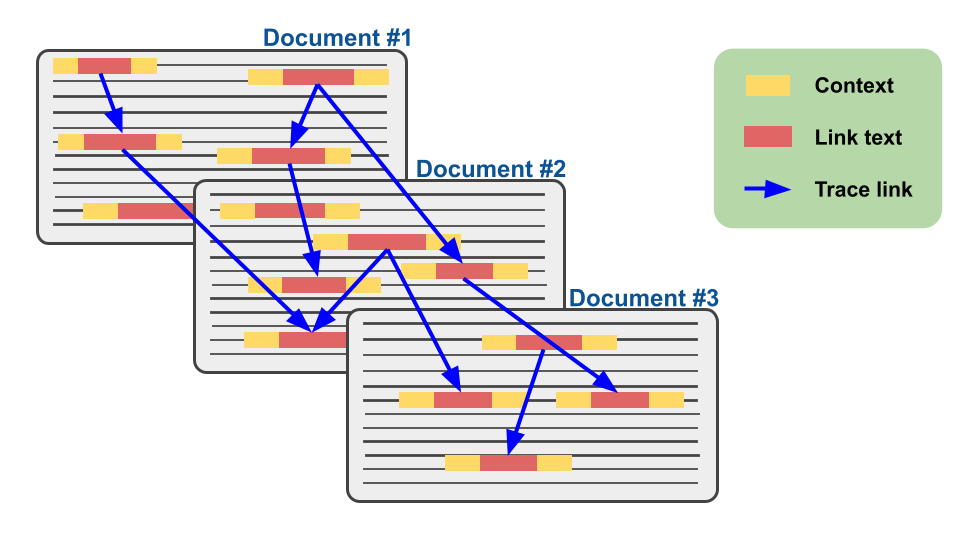
\includegraphics[width=0.7\textwidth]{use_graph}
  \caption{Random walk trace of locations visited by the document forager according to its traversal policy. These form a graph representing relevant entity links, which can be later used for prediction on a downstream task.}
\end{figure*}

During evaluation, we then measure how well the agent performed. Many loss functions are possible depending on the task, from a simple distance metric on a deleted fragment of code, to a more complex property (e.g. presence or absence of an error, or some internal state of the REPL) to be satisfied by interacting with the runtime environment. Many program analysis and repair tasks are amenable to the described setup, including defect, duplicate or vulnerability detection and correction.

\section{Method}

We fetch a dataset of random repositories on GitHub containing a mixture of filetypes representing both source code and natural language artifacts. Each project is indexed using a variable height radix tree, producing a multimap of prefix strings to a set of artifact, offset $(A, O)$ pairs in linear time.

 We initialize the policy network using a pretrained language model for the target languages. Starting at the site of the prediction task and conditioning on the context, the policy network draws K queries from its latent state. Querying the radix tree produces a set of matching locations within the project, and the process is repeated at each matching location using either a simple BFS traversal, or by expanding a subset of matching locations which are most promising, using MCTS with a finite horizon.

The rollout traces form a graph of related locations inside the project and their corresponding context embeddings, which become the GNN node features. Once the rollout ends, we run message passing on the resulting GNN for a fixed numbers of steps, then decode the graph embedding. Both the decoder, GNN weights, and policy network are trained end-to-end on the downstream task, e.g. code completion, defect detection or correction.

\section{Experiments}

In this work, we attempt to understand the relationship between entities in a software project. Our work seeks to answer the question: which artifacts in a software project are most useful for a given prediction task? We hypothesize that the policy network will learn to use both natural language and source code artifacts. If successful, this can be useful for both the prediction task itself, and knowledge graph extraction. Our research seeks to answer the following research questions. Can the agent can learn to:

\begin{enumerate}
  \item Navigate the project and locate contextually relevant artifacts?
  \item Comprehend the semantic content of contextually relevant artifacts?
  \item Apply the knowledge gathered to perform the assigned task?
\end{enumerate}

In our first experiment, we attempt to understand which queries the agent is performing when solving a programming task. Does it search for certain keywords in the context?

In our second experiment, we try to measure the information contained in various filetypes by ablating results in various filetypes. For trajectories which explore various filetypes such as Markdown or Java, what information gain do resources of these filetypes provide?

Our next steps are to build an RL environment which allows an agent to interact with a knowledge base and runtime environment. We will use an in-memory graph database to store and load project artifacts to and from the knowledge base. To model the agent, we will use the actions described above for navigating the environment, searching for text and reading documents, with a transformer-based internal state, pretrained on a corpus of projects in the same language. Finally, to evaluate the agent, we will generate problem instances and if necessary, use a JIT to rapidly validate generated code fragments.

  \bibliography{research_proposal}
  \bibliographystyle{plain}
\end{document}